\documentclass{standalone}
\standaloneconfig{border=2mm 2mm 2mm 2mm}
%Packages & Libraries
\usepackage{gensymb}
\usepackage{textcomp}
\usepackage{tikz}
\usepackage{tkz-euclide} 
\usetikzlibrary{patterns}

\begin{document}
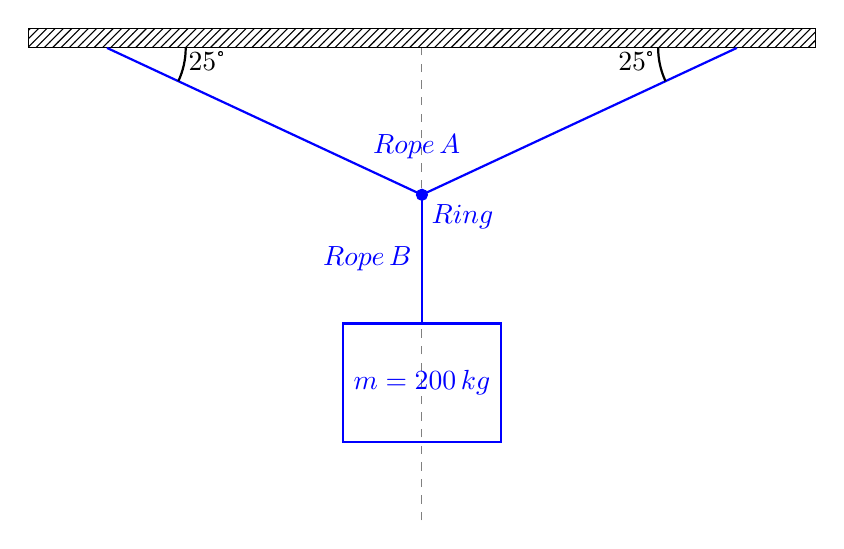
\begin{tikzpicture}
    %\draw [help lines] (0,0) grid (10,10);
    %\draw [help lines] (0,4) grid (10,10); %Modified grid
    % Axes
    \draw[dashed,gray] (5,4) -- (5,10); %y
    %\draw[dashed,gray] (0,5) -- (10,5); %x
    % Support
    \filldraw[pattern = north east lines] (0,10) rectangle ++(10,.25);      
    % Coordinates
    \coordinate (A) at (1,10);
    \coordinate (B) at (9,10);
    \coordinate (C) at (5,8.1347);
    % Sling
    \draw[blue, thick] (A) -- (C);
    \draw[thick] (2,10) arc (0:-25:1) node[anchor= south west]{$25\degree$};
    \draw[blue, thick] (B) -- (C) node[right] at (4.25,8.75) {$Rope\,A$};
    \draw[thick] (8,10) arc (180:205:1) node[anchor= south east]{$25\degree$};
    \draw[blue, thick] (C) -- (5,6.5) node[midway, below, left]{$Rope\,B$};
    \filldraw[blue] (C) circle (2pt) node[anchor= north west]{$Ring$};
    \draw[blue, thick] (4,5) rectangle (6,6.5) node[midway]{$m=200\,kg$} ;
\end{tikzpicture}
\end{document}
